\section{Relationenentwurf}
\label{sec:relationenentwurf}

\paragraph{Formalisierung Relationenmodell}
\begin{itemize}
	\item \textbf{Universum} \( U \): nichtleere endliche Menge \( U \)\\* (z.B. \( U= \{ \text{Name}, \text{Alter}, \text{Haarfarbe}, \dots \} \))
	\item \textbf{Attribut}: \( A \in U \)
	\item \textbf{Domäne} \( D \in \{ D_1, \dots, D_m \} \): endliche, nichtleere Menge \\* (z.B. \( D_1 = \{ 1,2,3,\dots \}, D_2 = \{ \text{schwarz}, \text{rot}, \text{blond} \} \))
	\item \textbf{Attributwert}: \( w \in \text{dom}(A) \) Attributwert für \( A \), \( \text{dom}: U \to D \): total definierte Funktion, \( \text{dom}(A) \) Domäne von \( A \) \\* (z.B. \( \text{dom}(\text{Haarfarbe}) = \{ \text{schwarz}, \text{rot}, \text{blond} \} \))
	\item \textbf{Relationenschema}: \( R \subseteq U \)
	\item \textbf{Tupel} (\( t \) in \( R = \{ A_1, \dots, A_n \} \)): \( t: R \to \bigcup_{i=1}^n D_i \)
	\item \textbf{Relation} (\( r \) über \( R = \{ A_1, \dots, A_n \} \)): endliche Menge von Tupeln \\* Notation: \( r(R) \) (Relation \( r \), Relationenschema \( R \))
	\begin{figure}[H]\centering\label{BeispielRelation}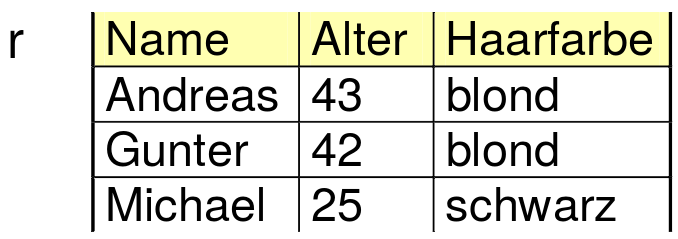
\includegraphics[width=.4\linewidth]{BeispielRelation}\end{figure}
	\item Beispiel: \\* \( R = \{ \text{Alter}, \text{Haarfarbe}, \text{Name} \} \) \\* \( r \) besteht aus Tupeln \( t_1, t_2, t_3 \); \( t_1(\text{Name}) = \text{``Andreas''} \) usw.
	\item \textbf{REL}: \( \text{REL}(R) = \{ r \mid r(R) \} \) \\* Menge aller Relationen über \( R \) sind \\* (\( r \) oben: \( r \in \text{REL}(\{ \text{Name}, \text{Alter}, \text{Haarfarbe} \}) \), \\* aber \( r \not \in \text{REL}(\{ \text{Name}, \text{Vorname} \}) \))
	\item \textbf{Datenbankschema}: \( S = \{ R_1, \dots, R_p \} \) \\* Menge von Relationenschemata
	\item \textbf{Datenbank} (\( d \) über \( S \)): Menge von Relationen \\* \( d = \{ r_1, \dots, r_p \} \) und \( r_i(R_i) \) \\* \( d(S) \) Datenbank \( d \) über \( S \)
\end{itemize}

\paragraph{Lokale Integritätsbedingung}
\begin{itemize}
	\item Abbildung aller möglichen Relationen zu einem Schema auf \lstinline{true} oder \lstinline{false}
	\item \( b: \text{REL}(R) \to \{ \) \lstinline{true}, \lstinline{false} \( \} \ (b \in B) \)
	\item \textbf{Erweitertes Relationenschema}: \( \mathcal{R} = (R, B) \)
	\item Abkürzung: \\* \( r(R) \) --- \( r \) ist Relation von \( R \) \\* \( r(\mathcal{R}) \) --- \( r \) ist Relation von \( R \), und \( b(r)= \) \lstinline{true} für alle \( b \in B \)
	\item \textbf{SAT}: \( \text{SAT}_R(B) = \{ r \mid r(\mathcal{R}) \} \) \\* Menge aller Relationen über erweitertem Relationenschema (SAT = \emph{satisfy})
\end{itemize}

\paragraph{Schlüssel}
\begin{itemize}
	\item Schlüssel und Fremdschlüssel einzige Integritätsbedingungen im relationalen Modell
	\item Schlüssel: Minimale identifizierende Attributmenge
	\item i.A. mehrere Schlüsselkandidaten, ein ausgezeichneter Primärschlüssel
	\item Fremdschlüssel \( X(R_1) \to Y(R_2) \): \\*
	\( \{ t(X) \mid t \in r_1 \} \subset \{ t(Y) \mid t \in r_2 \}  \) und $Y$ ist Schlüssel von $R_2$
\end{itemize}

\begin{fragen}
	\item Wie definieren wir \\*
		- Relation, \\*
		- Relationenschema, \\*
		- Integritätsbedingung?
\end{fragen}